\section{Softmax Function}
The softmax function is a mathematical function that converts a vector of real numbers into a vector of probabilities that sum to one. The softmax function is used in machine learning models to convert the output of a neural network into a probability distribution over multiple classes. The softmax function is defined as follows:
\begin{equation}
    \sigma(\vec{z})_j = \frac{e^{z_j}}{\sum_{k=1}^{K} e^{z_k}}
\end{equation}
Where:
\begin{itemize}[noitemsep]
    \item $\vec{z}$ is a vector of real numbers.
    \item $z_j$ is the $j^{th}$ element of the vector $\vec{z}$.
    \item $K$ is the number of classes.
    \item $\sigma(z)_j$ is the $j^{th}$ element of the output vector.
\end{itemize}
The figure \ref{fig:softmax} illustrates the softmax function for a vector of real numbers. Where each color represents an element in the input vector, where the height of the intersection of the line and the curve represents the percentage of the output vector.
\begin{figure}[H]
    \centering
    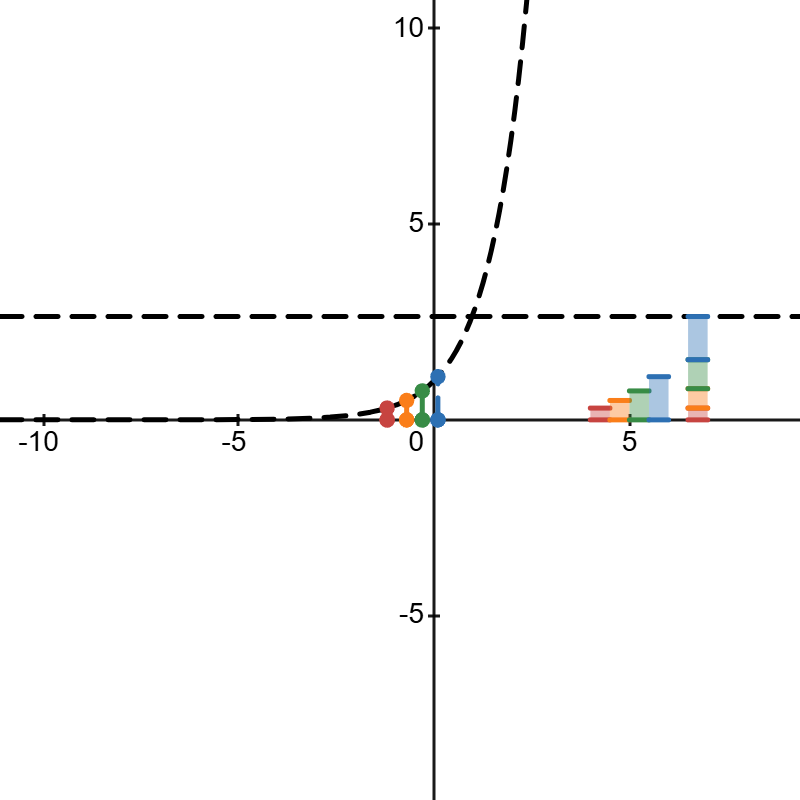
\includegraphics[width=0.5\textwidth]{assets/desmos-graph.png}
    \caption[Softmax Function]{Softmax Function}
    \label{fig:softmax}
\end{figure}
\subsection{Temperature Parameter}
The softmax function can be modified by introducing a temperature parameter $\tau$. The temperature parameter controls the entropy of the output distribution. A higher temperature parameter results in a more uniform distribution, while a lower temperature parameter results in a sharper distribution. The softmax function with a temperature parameter is defined as follows:
\begin{equation}
    \sigma(\vec{z})_j = \frac{e^{z_j/\tau}}{\sum_{k=1}^{K} e^{z_k/\tau}}
\end{equation}
Where:
\begin{itemize}[noitemsep]
    \item $\tau$ is the temperature parameter.
    \item $\vec{z}$ is a vector of real numbers.
    \item $z_j$ is the $j^{th}$ element of the vector $\vec{z}$.
    \item $K$ is the number of classes.
\end{itemize}
The figure \ref{fig:softmax_temperature} illustrates the difference between the softmax function with a temperature parameter and the softmax function without a temperature parameter. The figure shows that the softmax function with a temperature parameter results in a more uniform distribution.

\begin{figure}[H]
    \centering
    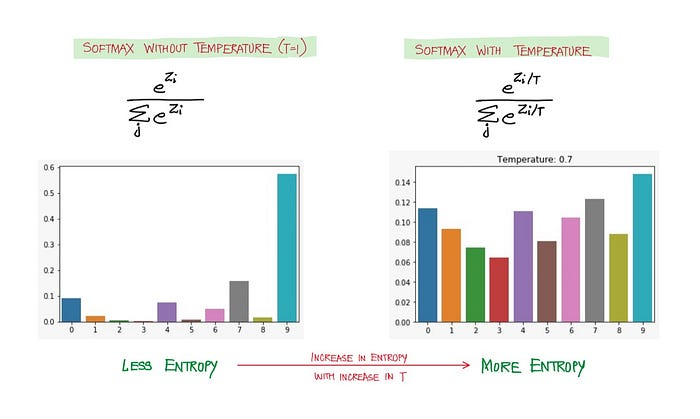
\includegraphics[width=0.5\textwidth]{assets/0_7xj72SjtNHvCMQlV.jpg}
    \caption[Softmax Function with Temperature Parameter]{Softmax Function with Temperature Parameter  \cite{Medium}}
    \label{fig:softmax_temperature}
\end{figure}